\documentclass{beamer}
\usepackage{graphicx}
\usetheme{Singapore}

\def\UrlBreaks{\do\/\do-} % URL breaks
\setbeamertemplate{caption}[numbered] % number figures
\setbeamertemplate{bibliography item}{\insertbiblabel} % bibliography numbers
\makeatletter
\newcommand*{\rom}[1]{\expandafter\@slowromancap\romannumeral #1@}
\makeatother

\title{Research Project Last-Layer Variational Inference}
\author{Philipp von Bachmann}
\institute{University of Tübingen}
\date{\today}



\begin{document}
        \begin{frame}
            \titlepage
        \end{frame}
        
        \section{Setup}
        \begin{frame}
            \frametitle{Idea}
            \begin{itemize}
                \item Setup: Deep Learning, neural network
                \item Problem: No confidence estimates
                \item Treat the last layer of the network as bayesian
                \item Train with Variational Inference
            \end{itemize}
        \end{frame}
        
        \section{Math and Training}
        \begin{frame}
            \frametitle{Variational Inference}
            $M$ model, $\theta$ network weights, $\phi$ parametrizes the variational distribution $q$ and $M$ of the prior $p$ over $\theta$\\
            ELBO formulation:
            \begin{equation*}
                \log{p(y \vert x, M)} \geq \sum_{i=1}^N \mathbb{E}_{q_{\phi}(\theta)}[\log{p(y_i \vert f_{\theta}(x_i), M)}] - D_{KL}(q_{\phi}(\theta) \Vert p_{M}(\theta))
            \end{equation*}
        \end{frame}

        \begin{frame}
            \frametitle{Training}
            \begin{equation*}
                \sum_{i=1}^N \mathbb{E}_{q_{\phi}(\theta)}[\log{p(y_i \vert f_{\theta}(x_i), M)}] - \tau \cdot D_{KL}(q_{\phi}(\theta) \Vert p_{M}(\theta))
            \end{equation*}
            \begin{itemize}
                \item $\tau$ controls balance of log-likelihood and KL Divergence
                \item approximate expectation with Monte-Carlo sampling
                \item different training modes:
                    \begin{itemize}
                        \item whole model jointly with VI
                        \item whole model with ''normal loss''
                        \item last layer with VI and keep other layers fixed
                    \end{itemize}
            \end{itemize}
        \end{frame}

        \begin{frame}
            \frametitle{Weight distribution}
            We use a multivariate Gaussian distribution for both $q$ and $p$.
            For the covariance we have following approximations:
            \begin{itemize}
                \item mean field, corresponds to diagonal Gaussian
                \item Kronecker-Factorization
                \item Full Covariance
            \end{itemize}
        \end{frame}


        \begin{frame}
            \frametitle{Hyperparameter Tuning}
            optimize model hyperparameters $M$
            \begin{itemize}
                \item normally done by Type-\rom{2} Maximum Likelihood estimation, $p(y \vert x, M)$
                \item ELBO gives lower bound on ML $\rightarrow$ maximize
                \item alternate between training model weights $\theta$ and hyperparameters $M$
            \end{itemize}

        \end{frame}

        \section{Examples}

        \begin{frame}
            \frametitle{Regression}
            \begin{figure}
                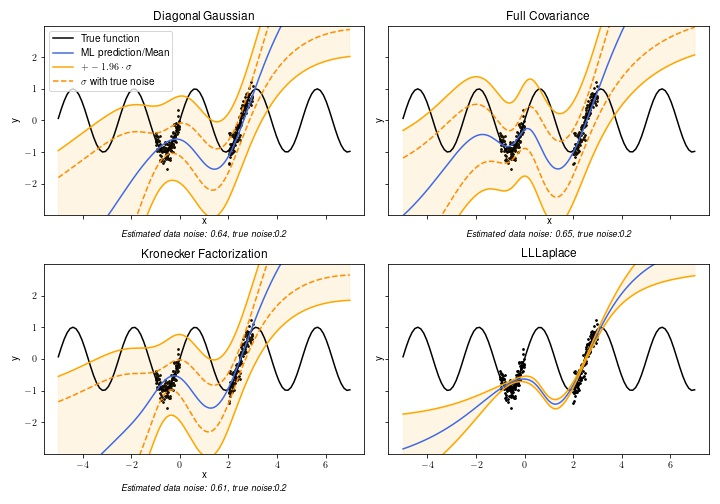
\includegraphics[width=\textwidth]{images/Regression/kernel_comparison.jpg}
            \end{figure}
        \end{frame}
        
        
        \begin{frame}
            
            \begin{itemize}
                \item  Calibration\\
                    \frametitle{MNIST}
                    \begin{figure}
                        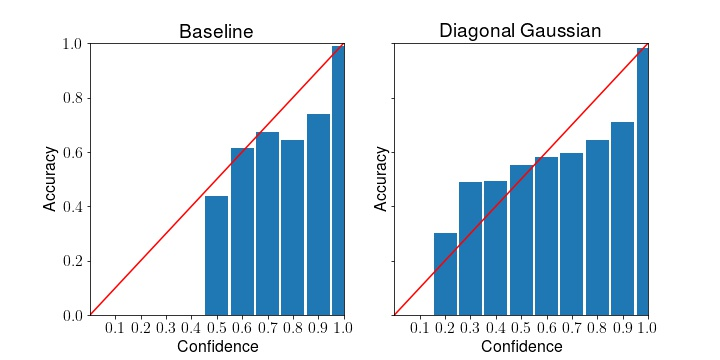
\includegraphics[width=0.8\textwidth]{images/MNIST/calibration.jpg}
                    \end{figure}
                \item Out of distribution confidence \\[10pt]
                    \centering
                    \scalebox{0.9}{
                        \begin{tabular}{c|c|c}
                            & Baseline & Diagonal\\
                            \hline
                            MNIST & 99 & 98 \\
                            MNIST horizontal flip & 87 & 72 \\
                            Fashion MNIST & 50 & 28
                        \end{tabular}
                    }

            \end{itemize}
        \end{frame}
        
        
        \begin{frame}
            \frametitle{Two Moons}
            \begin{figure}
                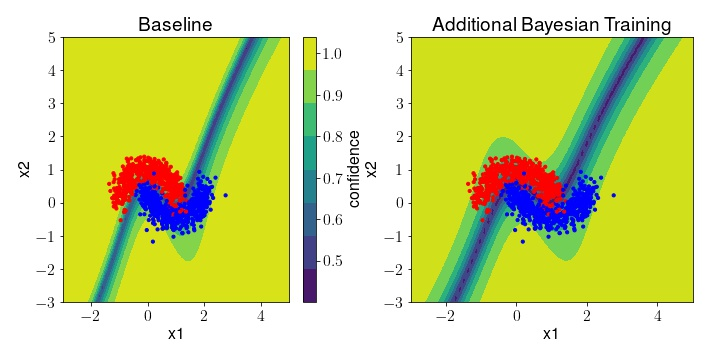
\includegraphics[width=\textwidth]{images/TwoMoons/comparison.jpg}
            \end{figure}
        \end{frame}
        
        \section{Next steps}
        \begin{frame}
            \frametitle{Next steps}
            \begin{itemize}
                \item more complex datasets (e.g. CIFAR-10)
                \item collapsed Variational Bound
                \item more kernels
            \end{itemize}
        \end{frame}


        % \begin{frame}
        %     \frametitle{Regression}
        %     add regression comparison of kernels here
        %     \begin{figure}
        %         \includegraphics[width=0.8\textwidth]{images/Regression/FullCov.jpg}
        %     \end{figure}
        % \end{frame}

        % \begin{frame}
        %     \frametitle{Classification: Two Moons}
        %     add non-bayesian vs best kernel comparison here, maybe vs laplace?
        %     \begin{columns}
        %         \column{0.5\textwidth}
        %         \begin{figure}
        %             \includegraphics[width=\textwidth]{images/TowMoons/Baseline.jpg}
        %         \end{figure}
        %         \column{0.5\textwidth}
        %         \begin{figure}
        %             \includegraphics[width=\textwidth]{images/TowMoons/Diagonal.jpg}
        %         \end{figure}
        %     \end{columns}
        % \end{frame}








\end{document}
